
% Default to the notebook output style

    


% Inherit from the specified cell style.




    
\documentclass[11pt]{article}

    
    
    \usepackage[T1]{fontenc}
    % Nicer default font (+ math font) than Computer Modern for most use cases
    \usepackage{mathpazo}

    % Basic figure setup, for now with no caption control since it's done
    % automatically by Pandoc (which extracts ![](path) syntax from Markdown).
    \usepackage{graphicx}
    % We will generate all images so they have a width \maxwidth. This means
    % that they will get their normal width if they fit onto the page, but
    % are scaled down if they would overflow the margins.
    \makeatletter
    \def\maxwidth{\ifdim\Gin@nat@width>\linewidth\linewidth
    \else\Gin@nat@width\fi}
    \makeatother
    \let\Oldincludegraphics\includegraphics
    % Set max figure width to be 80% of text width, for now hardcoded.
    \renewcommand{\includegraphics}[1]{\Oldincludegraphics[width=.8\maxwidth]{#1}}
    % Ensure that by default, figures have no caption (until we provide a
    % proper Figure object with a Caption API and a way to capture that
    % in the conversion process - todo).
    \usepackage{caption}
    \DeclareCaptionLabelFormat{nolabel}{}
    \captionsetup{labelformat=nolabel}

    \usepackage{adjustbox} % Used to constrain images to a maximum size 
    \usepackage{xcolor} % Allow colors to be defined
    \usepackage{enumerate} % Needed for markdown enumerations to work
    \usepackage{geometry} % Used to adjust the document margins
    \usepackage{amsmath} % Equations
    \usepackage{amssymb} % Equations
    \usepackage{textcomp} % defines textquotesingle
    % Hack from http://tex.stackexchange.com/a/47451/13684:
    \AtBeginDocument{%
        \def\PYZsq{\textquotesingle}% Upright quotes in Pygmentized code
    }
    \usepackage{upquote} % Upright quotes for verbatim code
    \usepackage{eurosym} % defines \euro
    \usepackage[mathletters]{ucs} % Extended unicode (utf-8) support
    \usepackage[utf8x]{inputenc} % Allow utf-8 characters in the tex document
    \usepackage{fancyvrb} % verbatim replacement that allows latex
    \usepackage{grffile} % extends the file name processing of package graphics 
                         % to support a larger range 
    % The hyperref package gives us a pdf with properly built
    % internal navigation ('pdf bookmarks' for the table of contents,
    % internal cross-reference links, web links for URLs, etc.)
    \usepackage{hyperref}
    \usepackage{longtable} % longtable support required by pandoc >1.10
    \usepackage{booktabs}  % table support for pandoc > 1.12.2
    \usepackage[inline]{enumitem} % IRkernel/repr support (it uses the enumerate* environment)
    \usepackage[normalem]{ulem} % ulem is needed to support strikethroughs (\sout)
                                % normalem makes italics be italics, not underlines
    

    
    
    % Colors for the hyperref package
    \definecolor{urlcolor}{rgb}{0,.145,.698}
    \definecolor{linkcolor}{rgb}{.71,0.21,0.01}
    \definecolor{citecolor}{rgb}{.12,.54,.11}

    % ANSI colors
    \definecolor{ansi-black}{HTML}{3E424D}
    \definecolor{ansi-black-intense}{HTML}{282C36}
    \definecolor{ansi-red}{HTML}{E75C58}
    \definecolor{ansi-red-intense}{HTML}{B22B31}
    \definecolor{ansi-green}{HTML}{00A250}
    \definecolor{ansi-green-intense}{HTML}{007427}
    \definecolor{ansi-yellow}{HTML}{DDB62B}
    \definecolor{ansi-yellow-intense}{HTML}{B27D12}
    \definecolor{ansi-blue}{HTML}{208FFB}
    \definecolor{ansi-blue-intense}{HTML}{0065CA}
    \definecolor{ansi-magenta}{HTML}{D160C4}
    \definecolor{ansi-magenta-intense}{HTML}{A03196}
    \definecolor{ansi-cyan}{HTML}{60C6C8}
    \definecolor{ansi-cyan-intense}{HTML}{258F8F}
    \definecolor{ansi-white}{HTML}{C5C1B4}
    \definecolor{ansi-white-intense}{HTML}{A1A6B2}

    % commands and environments needed by pandoc snippets
    % extracted from the output of `pandoc -s`
    \providecommand{\tightlist}{%
      \setlength{\itemsep}{0pt}\setlength{\parskip}{0pt}}
    \DefineVerbatimEnvironment{Highlighting}{Verbatim}{commandchars=\\\{\}}
    % Add ',fontsize=\small' for more characters per line
    \newenvironment{Shaded}{}{}
    \newcommand{\KeywordTok}[1]{\textcolor[rgb]{0.00,0.44,0.13}{\textbf{{#1}}}}
    \newcommand{\DataTypeTok}[1]{\textcolor[rgb]{0.56,0.13,0.00}{{#1}}}
    \newcommand{\DecValTok}[1]{\textcolor[rgb]{0.25,0.63,0.44}{{#1}}}
    \newcommand{\BaseNTok}[1]{\textcolor[rgb]{0.25,0.63,0.44}{{#1}}}
    \newcommand{\FloatTok}[1]{\textcolor[rgb]{0.25,0.63,0.44}{{#1}}}
    \newcommand{\CharTok}[1]{\textcolor[rgb]{0.25,0.44,0.63}{{#1}}}
    \newcommand{\StringTok}[1]{\textcolor[rgb]{0.25,0.44,0.63}{{#1}}}
    \newcommand{\CommentTok}[1]{\textcolor[rgb]{0.38,0.63,0.69}{\textit{{#1}}}}
    \newcommand{\OtherTok}[1]{\textcolor[rgb]{0.00,0.44,0.13}{{#1}}}
    \newcommand{\AlertTok}[1]{\textcolor[rgb]{1.00,0.00,0.00}{\textbf{{#1}}}}
    \newcommand{\FunctionTok}[1]{\textcolor[rgb]{0.02,0.16,0.49}{{#1}}}
    \newcommand{\RegionMarkerTok}[1]{{#1}}
    \newcommand{\ErrorTok}[1]{\textcolor[rgb]{1.00,0.00,0.00}{\textbf{{#1}}}}
    \newcommand{\NormalTok}[1]{{#1}}
    
    % Additional commands for more recent versions of Pandoc
    \newcommand{\ConstantTok}[1]{\textcolor[rgb]{0.53,0.00,0.00}{{#1}}}
    \newcommand{\SpecialCharTok}[1]{\textcolor[rgb]{0.25,0.44,0.63}{{#1}}}
    \newcommand{\VerbatimStringTok}[1]{\textcolor[rgb]{0.25,0.44,0.63}{{#1}}}
    \newcommand{\SpecialStringTok}[1]{\textcolor[rgb]{0.73,0.40,0.53}{{#1}}}
    \newcommand{\ImportTok}[1]{{#1}}
    \newcommand{\DocumentationTok}[1]{\textcolor[rgb]{0.73,0.13,0.13}{\textit{{#1}}}}
    \newcommand{\AnnotationTok}[1]{\textcolor[rgb]{0.38,0.63,0.69}{\textbf{\textit{{#1}}}}}
    \newcommand{\CommentVarTok}[1]{\textcolor[rgb]{0.38,0.63,0.69}{\textbf{\textit{{#1}}}}}
    \newcommand{\VariableTok}[1]{\textcolor[rgb]{0.10,0.09,0.49}{{#1}}}
    \newcommand{\ControlFlowTok}[1]{\textcolor[rgb]{0.00,0.44,0.13}{\textbf{{#1}}}}
    \newcommand{\OperatorTok}[1]{\textcolor[rgb]{0.40,0.40,0.40}{{#1}}}
    \newcommand{\BuiltInTok}[1]{{#1}}
    \newcommand{\ExtensionTok}[1]{{#1}}
    \newcommand{\PreprocessorTok}[1]{\textcolor[rgb]{0.74,0.48,0.00}{{#1}}}
    \newcommand{\AttributeTok}[1]{\textcolor[rgb]{0.49,0.56,0.16}{{#1}}}
    \newcommand{\InformationTok}[1]{\textcolor[rgb]{0.38,0.63,0.69}{\textbf{\textit{{#1}}}}}
    \newcommand{\WarningTok}[1]{\textcolor[rgb]{0.38,0.63,0.69}{\textbf{\textit{{#1}}}}}
    
    
    % Define a nice break command that doesn't care if a line doesn't already
    % exist.
    \def\br{\hspace*{\fill} \\* }
    % Math Jax compatability definitions
    \def\gt{>}
    \def\lt{<}
    % Document parameters
    \title{knn}
    
    
    

    % Pygments definitions
    
\makeatletter
\def\PY@reset{\let\PY@it=\relax \let\PY@bf=\relax%
    \let\PY@ul=\relax \let\PY@tc=\relax%
    \let\PY@bc=\relax \let\PY@ff=\relax}
\def\PY@tok#1{\csname PY@tok@#1\endcsname}
\def\PY@toks#1+{\ifx\relax#1\empty\else%
    \PY@tok{#1}\expandafter\PY@toks\fi}
\def\PY@do#1{\PY@bc{\PY@tc{\PY@ul{%
    \PY@it{\PY@bf{\PY@ff{#1}}}}}}}
\def\PY#1#2{\PY@reset\PY@toks#1+\relax+\PY@do{#2}}

\expandafter\def\csname PY@tok@w\endcsname{\def\PY@tc##1{\textcolor[rgb]{0.73,0.73,0.73}{##1}}}
\expandafter\def\csname PY@tok@c\endcsname{\let\PY@it=\textit\def\PY@tc##1{\textcolor[rgb]{0.25,0.50,0.50}{##1}}}
\expandafter\def\csname PY@tok@cp\endcsname{\def\PY@tc##1{\textcolor[rgb]{0.74,0.48,0.00}{##1}}}
\expandafter\def\csname PY@tok@k\endcsname{\let\PY@bf=\textbf\def\PY@tc##1{\textcolor[rgb]{0.00,0.50,0.00}{##1}}}
\expandafter\def\csname PY@tok@kp\endcsname{\def\PY@tc##1{\textcolor[rgb]{0.00,0.50,0.00}{##1}}}
\expandafter\def\csname PY@tok@kt\endcsname{\def\PY@tc##1{\textcolor[rgb]{0.69,0.00,0.25}{##1}}}
\expandafter\def\csname PY@tok@o\endcsname{\def\PY@tc##1{\textcolor[rgb]{0.40,0.40,0.40}{##1}}}
\expandafter\def\csname PY@tok@ow\endcsname{\let\PY@bf=\textbf\def\PY@tc##1{\textcolor[rgb]{0.67,0.13,1.00}{##1}}}
\expandafter\def\csname PY@tok@nb\endcsname{\def\PY@tc##1{\textcolor[rgb]{0.00,0.50,0.00}{##1}}}
\expandafter\def\csname PY@tok@nf\endcsname{\def\PY@tc##1{\textcolor[rgb]{0.00,0.00,1.00}{##1}}}
\expandafter\def\csname PY@tok@nc\endcsname{\let\PY@bf=\textbf\def\PY@tc##1{\textcolor[rgb]{0.00,0.00,1.00}{##1}}}
\expandafter\def\csname PY@tok@nn\endcsname{\let\PY@bf=\textbf\def\PY@tc##1{\textcolor[rgb]{0.00,0.00,1.00}{##1}}}
\expandafter\def\csname PY@tok@ne\endcsname{\let\PY@bf=\textbf\def\PY@tc##1{\textcolor[rgb]{0.82,0.25,0.23}{##1}}}
\expandafter\def\csname PY@tok@nv\endcsname{\def\PY@tc##1{\textcolor[rgb]{0.10,0.09,0.49}{##1}}}
\expandafter\def\csname PY@tok@no\endcsname{\def\PY@tc##1{\textcolor[rgb]{0.53,0.00,0.00}{##1}}}
\expandafter\def\csname PY@tok@nl\endcsname{\def\PY@tc##1{\textcolor[rgb]{0.63,0.63,0.00}{##1}}}
\expandafter\def\csname PY@tok@ni\endcsname{\let\PY@bf=\textbf\def\PY@tc##1{\textcolor[rgb]{0.60,0.60,0.60}{##1}}}
\expandafter\def\csname PY@tok@na\endcsname{\def\PY@tc##1{\textcolor[rgb]{0.49,0.56,0.16}{##1}}}
\expandafter\def\csname PY@tok@nt\endcsname{\let\PY@bf=\textbf\def\PY@tc##1{\textcolor[rgb]{0.00,0.50,0.00}{##1}}}
\expandafter\def\csname PY@tok@nd\endcsname{\def\PY@tc##1{\textcolor[rgb]{0.67,0.13,1.00}{##1}}}
\expandafter\def\csname PY@tok@s\endcsname{\def\PY@tc##1{\textcolor[rgb]{0.73,0.13,0.13}{##1}}}
\expandafter\def\csname PY@tok@sd\endcsname{\let\PY@it=\textit\def\PY@tc##1{\textcolor[rgb]{0.73,0.13,0.13}{##1}}}
\expandafter\def\csname PY@tok@si\endcsname{\let\PY@bf=\textbf\def\PY@tc##1{\textcolor[rgb]{0.73,0.40,0.53}{##1}}}
\expandafter\def\csname PY@tok@se\endcsname{\let\PY@bf=\textbf\def\PY@tc##1{\textcolor[rgb]{0.73,0.40,0.13}{##1}}}
\expandafter\def\csname PY@tok@sr\endcsname{\def\PY@tc##1{\textcolor[rgb]{0.73,0.40,0.53}{##1}}}
\expandafter\def\csname PY@tok@ss\endcsname{\def\PY@tc##1{\textcolor[rgb]{0.10,0.09,0.49}{##1}}}
\expandafter\def\csname PY@tok@sx\endcsname{\def\PY@tc##1{\textcolor[rgb]{0.00,0.50,0.00}{##1}}}
\expandafter\def\csname PY@tok@m\endcsname{\def\PY@tc##1{\textcolor[rgb]{0.40,0.40,0.40}{##1}}}
\expandafter\def\csname PY@tok@gh\endcsname{\let\PY@bf=\textbf\def\PY@tc##1{\textcolor[rgb]{0.00,0.00,0.50}{##1}}}
\expandafter\def\csname PY@tok@gu\endcsname{\let\PY@bf=\textbf\def\PY@tc##1{\textcolor[rgb]{0.50,0.00,0.50}{##1}}}
\expandafter\def\csname PY@tok@gd\endcsname{\def\PY@tc##1{\textcolor[rgb]{0.63,0.00,0.00}{##1}}}
\expandafter\def\csname PY@tok@gi\endcsname{\def\PY@tc##1{\textcolor[rgb]{0.00,0.63,0.00}{##1}}}
\expandafter\def\csname PY@tok@gr\endcsname{\def\PY@tc##1{\textcolor[rgb]{1.00,0.00,0.00}{##1}}}
\expandafter\def\csname PY@tok@ge\endcsname{\let\PY@it=\textit}
\expandafter\def\csname PY@tok@gs\endcsname{\let\PY@bf=\textbf}
\expandafter\def\csname PY@tok@gp\endcsname{\let\PY@bf=\textbf\def\PY@tc##1{\textcolor[rgb]{0.00,0.00,0.50}{##1}}}
\expandafter\def\csname PY@tok@go\endcsname{\def\PY@tc##1{\textcolor[rgb]{0.53,0.53,0.53}{##1}}}
\expandafter\def\csname PY@tok@gt\endcsname{\def\PY@tc##1{\textcolor[rgb]{0.00,0.27,0.87}{##1}}}
\expandafter\def\csname PY@tok@err\endcsname{\def\PY@bc##1{\setlength{\fboxsep}{0pt}\fcolorbox[rgb]{1.00,0.00,0.00}{1,1,1}{\strut ##1}}}
\expandafter\def\csname PY@tok@kc\endcsname{\let\PY@bf=\textbf\def\PY@tc##1{\textcolor[rgb]{0.00,0.50,0.00}{##1}}}
\expandafter\def\csname PY@tok@kd\endcsname{\let\PY@bf=\textbf\def\PY@tc##1{\textcolor[rgb]{0.00,0.50,0.00}{##1}}}
\expandafter\def\csname PY@tok@kn\endcsname{\let\PY@bf=\textbf\def\PY@tc##1{\textcolor[rgb]{0.00,0.50,0.00}{##1}}}
\expandafter\def\csname PY@tok@kr\endcsname{\let\PY@bf=\textbf\def\PY@tc##1{\textcolor[rgb]{0.00,0.50,0.00}{##1}}}
\expandafter\def\csname PY@tok@bp\endcsname{\def\PY@tc##1{\textcolor[rgb]{0.00,0.50,0.00}{##1}}}
\expandafter\def\csname PY@tok@fm\endcsname{\def\PY@tc##1{\textcolor[rgb]{0.00,0.00,1.00}{##1}}}
\expandafter\def\csname PY@tok@vc\endcsname{\def\PY@tc##1{\textcolor[rgb]{0.10,0.09,0.49}{##1}}}
\expandafter\def\csname PY@tok@vg\endcsname{\def\PY@tc##1{\textcolor[rgb]{0.10,0.09,0.49}{##1}}}
\expandafter\def\csname PY@tok@vi\endcsname{\def\PY@tc##1{\textcolor[rgb]{0.10,0.09,0.49}{##1}}}
\expandafter\def\csname PY@tok@vm\endcsname{\def\PY@tc##1{\textcolor[rgb]{0.10,0.09,0.49}{##1}}}
\expandafter\def\csname PY@tok@sa\endcsname{\def\PY@tc##1{\textcolor[rgb]{0.73,0.13,0.13}{##1}}}
\expandafter\def\csname PY@tok@sb\endcsname{\def\PY@tc##1{\textcolor[rgb]{0.73,0.13,0.13}{##1}}}
\expandafter\def\csname PY@tok@sc\endcsname{\def\PY@tc##1{\textcolor[rgb]{0.73,0.13,0.13}{##1}}}
\expandafter\def\csname PY@tok@dl\endcsname{\def\PY@tc##1{\textcolor[rgb]{0.73,0.13,0.13}{##1}}}
\expandafter\def\csname PY@tok@s2\endcsname{\def\PY@tc##1{\textcolor[rgb]{0.73,0.13,0.13}{##1}}}
\expandafter\def\csname PY@tok@sh\endcsname{\def\PY@tc##1{\textcolor[rgb]{0.73,0.13,0.13}{##1}}}
\expandafter\def\csname PY@tok@s1\endcsname{\def\PY@tc##1{\textcolor[rgb]{0.73,0.13,0.13}{##1}}}
\expandafter\def\csname PY@tok@mb\endcsname{\def\PY@tc##1{\textcolor[rgb]{0.40,0.40,0.40}{##1}}}
\expandafter\def\csname PY@tok@mf\endcsname{\def\PY@tc##1{\textcolor[rgb]{0.40,0.40,0.40}{##1}}}
\expandafter\def\csname PY@tok@mh\endcsname{\def\PY@tc##1{\textcolor[rgb]{0.40,0.40,0.40}{##1}}}
\expandafter\def\csname PY@tok@mi\endcsname{\def\PY@tc##1{\textcolor[rgb]{0.40,0.40,0.40}{##1}}}
\expandafter\def\csname PY@tok@il\endcsname{\def\PY@tc##1{\textcolor[rgb]{0.40,0.40,0.40}{##1}}}
\expandafter\def\csname PY@tok@mo\endcsname{\def\PY@tc##1{\textcolor[rgb]{0.40,0.40,0.40}{##1}}}
\expandafter\def\csname PY@tok@ch\endcsname{\let\PY@it=\textit\def\PY@tc##1{\textcolor[rgb]{0.25,0.50,0.50}{##1}}}
\expandafter\def\csname PY@tok@cm\endcsname{\let\PY@it=\textit\def\PY@tc##1{\textcolor[rgb]{0.25,0.50,0.50}{##1}}}
\expandafter\def\csname PY@tok@cpf\endcsname{\let\PY@it=\textit\def\PY@tc##1{\textcolor[rgb]{0.25,0.50,0.50}{##1}}}
\expandafter\def\csname PY@tok@c1\endcsname{\let\PY@it=\textit\def\PY@tc##1{\textcolor[rgb]{0.25,0.50,0.50}{##1}}}
\expandafter\def\csname PY@tok@cs\endcsname{\let\PY@it=\textit\def\PY@tc##1{\textcolor[rgb]{0.25,0.50,0.50}{##1}}}

\def\PYZbs{\char`\\}
\def\PYZus{\char`\_}
\def\PYZob{\char`\{}
\def\PYZcb{\char`\}}
\def\PYZca{\char`\^}
\def\PYZam{\char`\&}
\def\PYZlt{\char`\<}
\def\PYZgt{\char`\>}
\def\PYZsh{\char`\#}
\def\PYZpc{\char`\%}
\def\PYZdl{\char`\$}
\def\PYZhy{\char`\-}
\def\PYZsq{\char`\'}
\def\PYZdq{\char`\"}
\def\PYZti{\char`\~}
% for compatibility with earlier versions
\def\PYZat{@}
\def\PYZlb{[}
\def\PYZrb{]}
\makeatother


    % Exact colors from NB
    \definecolor{incolor}{rgb}{0.0, 0.0, 0.5}
    \definecolor{outcolor}{rgb}{0.545, 0.0, 0.0}



    
    % Prevent overflowing lines due to hard-to-break entities
    \sloppy 
    % Setup hyperref package
    \hypersetup{
      breaklinks=true,  % so long urls are correctly broken across lines
      colorlinks=true,
      urlcolor=urlcolor,
      linkcolor=linkcolor,
      citecolor=citecolor,
      }
    % Slightly bigger margins than the latex defaults
    
    \geometry{verbose,tmargin=1in,bmargin=1in,lmargin=1in,rmargin=1in}
    
    

    \begin{document}
    
    
    \maketitle
    
    

    
    \hypertarget{k-nearest-neighbor-knn-exercise}{%
\section{k-Nearest Neighbor (kNN)
exercise}\label{k-nearest-neighbor-knn-exercise}}

\emph{Complete and hand in this completed worksheet (including its
outputs and any supporting code outside of the worksheet) with your
assignment submission.}

The kNN classifier consists of two stages:

\begin{itemize}
\tightlist
\item
  During training, the classifier takes the training data and simply
  remembers it
\item
  During testing, kNN classifies every test image by comparing to all
  training images and transfering the labels of the k most similar
  training examples
\item
  The value of k is cross-validated
\end{itemize}

In this exercise you will implement these steps and understand the basic
Image Classification pipeline, cross-validation, and gain proficiency in
writing efficient, vectorized code.

    \begin{Verbatim}[commandchars=\\\{\}]
{\color{incolor}In [{\color{incolor}1}]:} \PY{c+c1}{\PYZsh{} Run some setup code for this notebook.}
        
        \PY{k+kn}{from} \PY{n+nn}{\PYZus{}\PYZus{}future\PYZus{}\PYZus{}} \PY{k}{import} \PY{n}{print\PYZus{}function}
        \PY{k+kn}{import} \PY{n+nn}{random}
        \PY{k+kn}{import} \PY{n+nn}{numpy} \PY{k}{as} \PY{n+nn}{np}
        \PY{k+kn}{from} \PY{n+nn}{data\PYZus{}utils} \PY{k}{import} \PY{n}{load\PYZus{}CIFAR10}
        \PY{k+kn}{import} \PY{n+nn}{matplotlib}\PY{n+nn}{.}\PY{n+nn}{pyplot} \PY{k}{as} \PY{n+nn}{plt}  
        
        \PY{c+c1}{\PYZsh{} This is a bit of magic to make matplotlib figures appear inline in the notebook}
        \PY{c+c1}{\PYZsh{} rather than in a new window.}
        \PY{o}{\PYZpc{}}\PY{k}{matplotlib} inline
        \PY{n}{plt}\PY{o}{.}\PY{n}{rcParams}\PY{p}{[}\PY{l+s+s1}{\PYZsq{}}\PY{l+s+s1}{figure.figsize}\PY{l+s+s1}{\PYZsq{}}\PY{p}{]} \PY{o}{=} \PY{p}{(}\PY{l+m+mf}{10.0}\PY{p}{,} \PY{l+m+mf}{8.0}\PY{p}{)} \PY{c+c1}{\PYZsh{} set default size of plots}
        \PY{n}{plt}\PY{o}{.}\PY{n}{rcParams}\PY{p}{[}\PY{l+s+s1}{\PYZsq{}}\PY{l+s+s1}{image.interpolation}\PY{l+s+s1}{\PYZsq{}}\PY{p}{]} \PY{o}{=} \PY{l+s+s1}{\PYZsq{}}\PY{l+s+s1}{nearest}\PY{l+s+s1}{\PYZsq{}}
        \PY{n}{plt}\PY{o}{.}\PY{n}{rcParams}\PY{p}{[}\PY{l+s+s1}{\PYZsq{}}\PY{l+s+s1}{image.cmap}\PY{l+s+s1}{\PYZsq{}}\PY{p}{]} \PY{o}{=} \PY{l+s+s1}{\PYZsq{}}\PY{l+s+s1}{gray}\PY{l+s+s1}{\PYZsq{}}
        
        \PY{c+c1}{\PYZsh{} Some more magic so that the notebook will reload external python modules;}
        \PY{c+c1}{\PYZsh{} see http://stackoverflow.com/questions/1907993/autoreload\PYZhy{}of\PYZhy{}modules\PYZhy{}in\PYZhy{}ipython}
        \PY{o}{\PYZpc{}}\PY{k}{load\PYZus{}ext} autoreload
        \PY{o}{\PYZpc{}}\PY{k}{autoreload} 2
\end{Verbatim}


    \begin{Verbatim}[commandchars=\\\{\}]
{\color{incolor}In [{\color{incolor}2}]:} \PY{k}{def} \PY{n+nf}{rel\PYZus{}error}\PY{p}{(}\PY{n}{out}\PY{p}{,} \PY{n}{correct\PYZus{}out}\PY{p}{)}\PY{p}{:}
            \PY{k}{return} \PY{n}{np}\PY{o}{.}\PY{n}{sum}\PY{p}{(}\PY{n+nb}{abs}\PY{p}{(}\PY{n}{out} \PY{o}{\PYZhy{}} \PY{n}{correct\PYZus{}out}\PY{p}{)} \PY{o}{/} \PY{p}{(}\PY{n+nb}{abs}\PY{p}{(}\PY{n}{out}\PY{p}{)} \PY{o}{+} \PY{n+nb}{abs}\PY{p}{(}\PY{n}{correct\PYZus{}out}\PY{p}{)}\PY{p}{)}\PY{p}{)}
\end{Verbatim}


    \begin{Verbatim}[commandchars=\\\{\}]
{\color{incolor}In [{\color{incolor}3}]:} \PY{c+c1}{\PYZsh{} Load the raw CIFAR\PYZhy{}10 data.}
        \PY{n}{cifar10\PYZus{}dir} \PY{o}{=} \PY{l+s+s1}{\PYZsq{}}\PY{l+s+s1}{datasets/cifar\PYZhy{}10\PYZhy{}batches\PYZhy{}py}\PY{l+s+s1}{\PYZsq{}}
        \PY{n}{X\PYZus{}train}\PY{p}{,} \PY{n}{y\PYZus{}train}\PY{p}{,} \PY{n}{X\PYZus{}test}\PY{p}{,} \PY{n}{y\PYZus{}test} \PY{o}{=} \PY{n}{load\PYZus{}CIFAR10}\PY{p}{(}\PY{n}{cifar10\PYZus{}dir}\PY{p}{)}
        
        \PY{c+c1}{\PYZsh{} As a sanity check, we print out the size of the training and test data.}
        \PY{n+nb}{print}\PY{p}{(}\PY{l+s+s1}{\PYZsq{}}\PY{l+s+s1}{Training data shape: }\PY{l+s+s1}{\PYZsq{}}\PY{p}{,} \PY{n}{X\PYZus{}train}\PY{o}{.}\PY{n}{shape}\PY{p}{)}
        \PY{n+nb}{print}\PY{p}{(}\PY{l+s+s1}{\PYZsq{}}\PY{l+s+s1}{Training labels shape: }\PY{l+s+s1}{\PYZsq{}}\PY{p}{,} \PY{n}{y\PYZus{}train}\PY{o}{.}\PY{n}{shape}\PY{p}{)}
        \PY{n+nb}{print}\PY{p}{(}\PY{l+s+s1}{\PYZsq{}}\PY{l+s+s1}{Test data shape: }\PY{l+s+s1}{\PYZsq{}}\PY{p}{,} \PY{n}{X\PYZus{}test}\PY{o}{.}\PY{n}{shape}\PY{p}{)}
        \PY{n+nb}{print}\PY{p}{(}\PY{l+s+s1}{\PYZsq{}}\PY{l+s+s1}{Test labels shape: }\PY{l+s+s1}{\PYZsq{}}\PY{p}{,} \PY{n}{y\PYZus{}test}\PY{o}{.}\PY{n}{shape}\PY{p}{)}
\end{Verbatim}


    \begin{Verbatim}[commandchars=\\\{\}]
Training data shape:  (50000, 32, 32, 3)
Training labels shape:  (50000,)
Test data shape:  (10000, 32, 32, 3)
Test labels shape:  (10000,)

    \end{Verbatim}

    \begin{Verbatim}[commandchars=\\\{\}]
{\color{incolor}In [{\color{incolor}4}]:} \PY{c+c1}{\PYZsh{} Visualize some examples from the dataset.}
        \PY{c+c1}{\PYZsh{} We show a few examples of training images from each class.}
        \PY{n}{classes} \PY{o}{=} \PY{p}{[}\PY{l+s+s1}{\PYZsq{}}\PY{l+s+s1}{plane}\PY{l+s+s1}{\PYZsq{}}\PY{p}{,} \PY{l+s+s1}{\PYZsq{}}\PY{l+s+s1}{car}\PY{l+s+s1}{\PYZsq{}}\PY{p}{,} \PY{l+s+s1}{\PYZsq{}}\PY{l+s+s1}{bird}\PY{l+s+s1}{\PYZsq{}}\PY{p}{,} \PY{l+s+s1}{\PYZsq{}}\PY{l+s+s1}{cat}\PY{l+s+s1}{\PYZsq{}}\PY{p}{,} \PY{l+s+s1}{\PYZsq{}}\PY{l+s+s1}{deer}\PY{l+s+s1}{\PYZsq{}}\PY{p}{,} \PY{l+s+s1}{\PYZsq{}}\PY{l+s+s1}{dog}\PY{l+s+s1}{\PYZsq{}}\PY{p}{,} \PY{l+s+s1}{\PYZsq{}}\PY{l+s+s1}{frog}\PY{l+s+s1}{\PYZsq{}}\PY{p}{,} \PY{l+s+s1}{\PYZsq{}}\PY{l+s+s1}{horse}\PY{l+s+s1}{\PYZsq{}}\PY{p}{,} \PY{l+s+s1}{\PYZsq{}}\PY{l+s+s1}{ship}\PY{l+s+s1}{\PYZsq{}}\PY{p}{,} \PY{l+s+s1}{\PYZsq{}}\PY{l+s+s1}{truck}\PY{l+s+s1}{\PYZsq{}}\PY{p}{]}
        \PY{n}{num\PYZus{}classes} \PY{o}{=} \PY{n+nb}{len}\PY{p}{(}\PY{n}{classes}\PY{p}{)}
        \PY{n}{samples\PYZus{}per\PYZus{}class} \PY{o}{=} \PY{l+m+mi}{7}
        \PY{k}{for} \PY{n}{y}\PY{p}{,} \PY{n+nb+bp}{cls} \PY{o+ow}{in} \PY{n+nb}{enumerate}\PY{p}{(}\PY{n}{classes}\PY{p}{)}\PY{p}{:}
            \PY{n}{idxs} \PY{o}{=} \PY{n}{np}\PY{o}{.}\PY{n}{flatnonzero}\PY{p}{(}\PY{n}{y\PYZus{}train} \PY{o}{==} \PY{n}{y}\PY{p}{)}
            \PY{n}{idxs} \PY{o}{=} \PY{n}{np}\PY{o}{.}\PY{n}{random}\PY{o}{.}\PY{n}{choice}\PY{p}{(}\PY{n}{idxs}\PY{p}{,} \PY{n}{samples\PYZus{}per\PYZus{}class}\PY{p}{,} \PY{n}{replace}\PY{o}{=}\PY{k+kc}{False}\PY{p}{)}
            \PY{k}{for} \PY{n}{i}\PY{p}{,} \PY{n}{idx} \PY{o+ow}{in} \PY{n+nb}{enumerate}\PY{p}{(}\PY{n}{idxs}\PY{p}{)}\PY{p}{:}
                \PY{n}{plt\PYZus{}idx} \PY{o}{=} \PY{n}{i} \PY{o}{*} \PY{n}{num\PYZus{}classes} \PY{o}{+} \PY{n}{y} \PY{o}{+} \PY{l+m+mi}{1}
                \PY{n}{plt}\PY{o}{.}\PY{n}{subplot}\PY{p}{(}\PY{n}{samples\PYZus{}per\PYZus{}class}\PY{p}{,} \PY{n}{num\PYZus{}classes}\PY{p}{,} \PY{n}{plt\PYZus{}idx}\PY{p}{)}
                \PY{n}{plt}\PY{o}{.}\PY{n}{imshow}\PY{p}{(}\PY{n}{X\PYZus{}train}\PY{p}{[}\PY{n}{idx}\PY{p}{]}\PY{o}{.}\PY{n}{astype}\PY{p}{(}\PY{l+s+s1}{\PYZsq{}}\PY{l+s+s1}{uint8}\PY{l+s+s1}{\PYZsq{}}\PY{p}{)}\PY{p}{)}
                \PY{n}{plt}\PY{o}{.}\PY{n}{axis}\PY{p}{(}\PY{l+s+s1}{\PYZsq{}}\PY{l+s+s1}{off}\PY{l+s+s1}{\PYZsq{}}\PY{p}{)}
                \PY{k}{if} \PY{n}{i} \PY{o}{==} \PY{l+m+mi}{0}\PY{p}{:}
                    \PY{n}{plt}\PY{o}{.}\PY{n}{title}\PY{p}{(}\PY{n+nb+bp}{cls}\PY{p}{)}
        \PY{n}{plt}\PY{o}{.}\PY{n}{show}\PY{p}{(}\PY{p}{)}
\end{Verbatim}


    \begin{center}
    \adjustimage{max size={0.9\linewidth}{0.9\paperheight}}{output_4_0.png}
    \end{center}
    { \hspace*{\fill} \\}
    
    \begin{Verbatim}[commandchars=\\\{\}]
{\color{incolor}In [{\color{incolor}5}]:} \PY{c+c1}{\PYZsh{} Subsample the data for more efficient code execution in this exercise}
        \PY{n}{num\PYZus{}training} \PY{o}{=} \PY{l+m+mi}{5000}
        \PY{n}{mask} \PY{o}{=} \PY{n+nb}{range}\PY{p}{(}\PY{n}{num\PYZus{}training}\PY{p}{)}
        
        \PY{n}{X\PYZus{}train} \PY{o}{=} \PY{n}{X\PYZus{}train}\PY{p}{[}\PY{n}{mask}\PY{p}{]}
        \PY{n}{y\PYZus{}train} \PY{o}{=} \PY{n}{y\PYZus{}train}\PY{p}{[}\PY{n}{mask}\PY{p}{]}
        
        \PY{n}{num\PYZus{}test} \PY{o}{=} \PY{l+m+mi}{500}
        \PY{n}{mask} \PY{o}{=} \PY{n+nb}{range}\PY{p}{(}\PY{n}{num\PYZus{}test}\PY{p}{)}
        \PY{n}{X\PYZus{}test} \PY{o}{=} \PY{n}{X\PYZus{}test}\PY{p}{[}\PY{n}{mask}\PY{p}{]}
        \PY{n}{y\PYZus{}test} \PY{o}{=} \PY{n}{y\PYZus{}test}\PY{p}{[}\PY{n}{mask}\PY{p}{]}
\end{Verbatim}


    \begin{Verbatim}[commandchars=\\\{\}]
{\color{incolor}In [{\color{incolor}6}]:} \PY{c+c1}{\PYZsh{} Reshape the image data into rows}
        \PY{n}{X\PYZus{}train} \PY{o}{=} \PY{n}{np}\PY{o}{.}\PY{n}{reshape}\PY{p}{(}\PY{n}{X\PYZus{}train}\PY{p}{,} \PY{p}{(}\PY{n}{X\PYZus{}train}\PY{o}{.}\PY{n}{shape}\PY{p}{[}\PY{l+m+mi}{0}\PY{p}{]}\PY{p}{,} \PY{o}{\PYZhy{}}\PY{l+m+mi}{1}\PY{p}{)}\PY{p}{)}
        \PY{n}{X\PYZus{}test} \PY{o}{=} \PY{n}{np}\PY{o}{.}\PY{n}{reshape}\PY{p}{(}\PY{n}{X\PYZus{}test}\PY{p}{,} \PY{p}{(}\PY{n}{X\PYZus{}test}\PY{o}{.}\PY{n}{shape}\PY{p}{[}\PY{l+m+mi}{0}\PY{p}{]}\PY{p}{,} \PY{o}{\PYZhy{}}\PY{l+m+mi}{1}\PY{p}{)}\PY{p}{)}
        \PY{n+nb}{print}\PY{p}{(}\PY{n}{X\PYZus{}train}\PY{o}{.}\PY{n}{shape}\PY{p}{,} \PY{n}{X\PYZus{}test}\PY{o}{.}\PY{n}{shape}\PY{p}{)}
\end{Verbatim}


    \begin{Verbatim}[commandchars=\\\{\}]
(5000, 3072) (500, 3072)

    \end{Verbatim}

    \begin{Verbatim}[commandchars=\\\{\}]
{\color{incolor}In [{\color{incolor}7}]:} \PY{k+kn}{from} \PY{n+nn}{classifiers} \PY{k}{import} \PY{n}{KNearestNeighbor}
        
        \PY{c+c1}{\PYZsh{} Create a kNN classifier instance. }
        \PY{c+c1}{\PYZsh{} Remember that training a kNN classifier is a noop: }
        \PY{c+c1}{\PYZsh{} the Classifier simply remembers the data and does no further processing }
        \PY{n}{classifier} \PY{o}{=} \PY{n}{KNearestNeighbor}\PY{p}{(}\PY{p}{)}
        \PY{n}{classifier}\PY{o}{.}\PY{n}{train}\PY{p}{(}\PY{n}{X\PYZus{}train}\PY{p}{,} \PY{n}{y\PYZus{}train}\PY{p}{)}
\end{Verbatim}


    We would now like to classify the test data with the kNN classifier.
Recall that we can break down this process into two steps:

\begin{enumerate}
\def\labelenumi{\arabic{enumi}.}
\tightlist
\item
  First we must compute the distances between all test examples and all
  train examples.
\item
  Given these distances, for each test example we find the k nearest
  examples and have them vote for the label
\end{enumerate}

Lets begin with computing the distance matrix between all training and
test examples. For example, if there are \textbf{Ntr} training examples
and \textbf{Nte} test examples, this stage should result in a
\textbf{Nte x Ntr} matrix where each element (i,j) is the distance
between the i-th test and j-th train example.

First, open \texttt{classifiers/k\_nearest\_neighbor.py} and implement
the function \texttt{compute\_distances\_two\_loops} that uses a (very
inefficient) double loop over all pairs of (test, train) examples and
computes the distance matrix one element at a time.

    \begin{Verbatim}[commandchars=\\\{\}]
{\color{incolor}In [{\color{incolor}8}]:} \PY{c+c1}{\PYZsh{} Open classifiers/k\PYZus{}nearest\PYZus{}neighbor.py and implement}
        \PY{c+c1}{\PYZsh{} compute\PYZus{}distances\PYZus{}two\PYZus{}loops.}
        
        \PY{c+c1}{\PYZsh{} Test your implementation:}
        \PY{n}{dists} \PY{o}{=} \PY{n}{classifier}\PY{o}{.}\PY{n}{compute\PYZus{}distances\PYZus{}two\PYZus{}loops}\PY{p}{(}\PY{n}{X\PYZus{}test}\PY{p}{)}
        \PY{n+nb}{print}\PY{p}{(}\PY{n}{dists}\PY{o}{.}\PY{n}{shape}\PY{p}{)}
\end{Verbatim}


    \begin{Verbatim}[commandchars=\\\{\}]
(500, 5000)

    \end{Verbatim}

    \begin{Verbatim}[commandchars=\\\{\}]
{\color{incolor}In [{\color{incolor}9}]:} \PY{c+c1}{\PYZsh{} We can visualize the distance matrix: each row is a single test example and}
        \PY{c+c1}{\PYZsh{} its distances to training examples}
        \PY{n}{plt}\PY{o}{.}\PY{n}{imshow}\PY{p}{(}\PY{n}{dists}\PY{p}{,} \PY{n}{interpolation}\PY{o}{=}\PY{l+s+s1}{\PYZsq{}}\PY{l+s+s1}{none}\PY{l+s+s1}{\PYZsq{}}\PY{p}{)}
        \PY{n}{plt}\PY{o}{.}\PY{n}{show}\PY{p}{(}\PY{p}{)}
\end{Verbatim}


    \begin{center}
    \adjustimage{max size={0.9\linewidth}{0.9\paperheight}}{output_10_0.png}
    \end{center}
    { \hspace*{\fill} \\}
    
    \textbf{Inline Question \#1:} Notice the structured patterns in the
distance matrix, where some rows or columns are visible brighter. (Note
that with the default color scheme black indicates low distances while
white indicates high distances.)

\begin{itemize}
\tightlist
\item
  What in the data is the cause behind the distinctly bright rows?
\item
  What causes the columns?
\end{itemize}

    \textbf{Your Answer}: - This data point in testing data has high
distances to the training data. - This data point in training data has
high distances to the testing data.

    \begin{Verbatim}[commandchars=\\\{\}]
{\color{incolor}In [{\color{incolor}10}]:} \PY{c+c1}{\PYZsh{} Now implement the function predict\PYZus{}labels and run the code below:}
         \PY{c+c1}{\PYZsh{} We use k = 1 (which is Nearest Neighbor).}
         \PY{n}{y\PYZus{}test\PYZus{}pred} \PY{o}{=} \PY{n}{classifier}\PY{o}{.}\PY{n}{predict\PYZus{}labels}\PY{p}{(}\PY{n}{dists}\PY{p}{,} \PY{n}{k}\PY{o}{=}\PY{l+m+mi}{1}\PY{p}{)}
         
         \PY{c+c1}{\PYZsh{} Compute and print the fraction of correctly predicted examples}
         \PY{n}{num\PYZus{}correct} \PY{o}{=} \PY{n}{np}\PY{o}{.}\PY{n}{sum}\PY{p}{(}\PY{n}{y\PYZus{}test\PYZus{}pred} \PY{o}{==} \PY{n}{y\PYZus{}test}\PY{p}{)}
         \PY{n}{accuracy} \PY{o}{=} \PY{n+nb}{float}\PY{p}{(}\PY{n}{num\PYZus{}correct}\PY{p}{)} \PY{o}{/} \PY{n}{num\PYZus{}test}
         \PY{n+nb}{print}\PY{p}{(}\PY{l+s+s1}{\PYZsq{}}\PY{l+s+s1}{Got }\PY{l+s+si}{\PYZpc{}d}\PY{l+s+s1}{ / }\PY{l+s+si}{\PYZpc{}d}\PY{l+s+s1}{ correct =\PYZgt{} accuracy: }\PY{l+s+si}{\PYZpc{}f}\PY{l+s+s1}{\PYZsq{}} \PY{o}{\PYZpc{}} \PY{p}{(}\PY{n}{num\PYZus{}correct}\PY{p}{,} \PY{n}{num\PYZus{}test}\PY{p}{,} \PY{n}{accuracy}\PY{p}{)}\PY{p}{)}
\end{Verbatim}


    \begin{Verbatim}[commandchars=\\\{\}]
Got 137 / 500 correct => accuracy: 0.274000

    \end{Verbatim}

    You should expect to see approximately \texttt{27\%} accuracy. Now lets
try out a larger \texttt{k}, say \texttt{k\ =\ 5}:

    \begin{Verbatim}[commandchars=\\\{\}]
{\color{incolor}In [{\color{incolor}11}]:} \PY{n}{y\PYZus{}test\PYZus{}pred} \PY{o}{=} \PY{n}{classifier}\PY{o}{.}\PY{n}{predict\PYZus{}labels}\PY{p}{(}\PY{n}{dists}\PY{p}{,} \PY{n}{k}\PY{o}{=}\PY{l+m+mi}{5}\PY{p}{)}
         \PY{n}{num\PYZus{}correct} \PY{o}{=} \PY{n}{np}\PY{o}{.}\PY{n}{sum}\PY{p}{(}\PY{n}{y\PYZus{}test\PYZus{}pred} \PY{o}{==} \PY{n}{y\PYZus{}test}\PY{p}{)}
         \PY{n}{accuracy} \PY{o}{=} \PY{n+nb}{float}\PY{p}{(}\PY{n}{num\PYZus{}correct}\PY{p}{)} \PY{o}{/} \PY{n}{num\PYZus{}test}
         \PY{n+nb}{print}\PY{p}{(}\PY{l+s+s1}{\PYZsq{}}\PY{l+s+s1}{Got }\PY{l+s+si}{\PYZpc{}d}\PY{l+s+s1}{ / }\PY{l+s+si}{\PYZpc{}d}\PY{l+s+s1}{ correct =\PYZgt{} accuracy: }\PY{l+s+si}{\PYZpc{}f}\PY{l+s+s1}{\PYZsq{}} \PY{o}{\PYZpc{}} \PY{p}{(}\PY{n}{num\PYZus{}correct}\PY{p}{,} \PY{n}{num\PYZus{}test}\PY{p}{,} \PY{n}{accuracy}\PY{p}{)}\PY{p}{)}
\end{Verbatim}


    \begin{Verbatim}[commandchars=\\\{\}]
Got 139 / 500 correct => accuracy: 0.278000

    \end{Verbatim}

    You should expect to see a slightly better performance than with
\texttt{k\ =\ 1}.

    \hypertarget{frobenius-norm}{%
\subsection{Frobenius Norm}\label{frobenius-norm}}

To ensure that our vectorized implementation is correct, we make sure
that it agrees with the naive implementation. There are many ways to
decide whether two matrices are similar; one of the simplest is
\textbf{the Frobenius norm}. * Frobenius norm of \(m\times n\) matrix
\(A\) is defined as the square root of the sum of the absolute squares
of its elements,:
\[\|A\|_F=\sqrt{\sum\limits_{i=1}^m\sum\limits_{j=1}^nA_{ij}^2}\]

    \begin{Verbatim}[commandchars=\\\{\}]
{\color{incolor}In [{\color{incolor}12}]:} \PY{k}{def} \PY{n+nf}{Frobenius\PYZus{}norm}\PY{p}{(}\PY{n}{A}\PY{p}{)}\PY{p}{:}
             \PY{n}{Fnorm} \PY{o}{=} \PY{l+m+mi}{0}
             \PY{c+c1}{\PYZsh{}\PYZsh{}\PYZsh{}\PYZsh{}\PYZsh{}\PYZsh{}\PYZsh{}\PYZsh{}\PYZsh{}\PYZsh{}\PYZsh{}\PYZsh{}\PYZsh{}\PYZsh{}\PYZsh{}\PYZsh{}\PYZsh{}\PYZsh{}\PYZsh{}\PYZsh{}\PYZsh{}\PYZsh{}\PYZsh{}\PYZsh{}\PYZsh{}\PYZsh{}\PYZsh{}\PYZsh{}\PYZsh{}\PYZsh{}\PYZsh{}\PYZsh{}\PYZsh{}\PYZsh{}\PYZsh{}\PYZsh{}\PYZsh{}\PYZsh{}\PYZsh{}\PYZsh{}\PYZsh{}\PYZsh{}\PYZsh{}\PYZsh{}\PYZsh{}\PYZsh{}\PYZsh{}\PYZsh{}\PYZsh{}\PYZsh{}\PYZsh{}\PYZsh{}\PYZsh{}\PYZsh{}\PYZsh{}\PYZsh{}\PYZsh{}\PYZsh{}\PYZsh{}\PYZsh{}\PYZsh{}\PYZsh{}\PYZsh{}\PYZsh{}\PYZsh{}\PYZsh{}\PYZsh{}\PYZsh{}\PYZsh{}\PYZsh{}\PYZsh{}\PYZsh{}\PYZsh{}\PYZsh{}\PYZsh{}\PYZsh{}\PYZsh{}\PYZsh{}\PYZsh{}\PYZsh{}}
             \PY{c+c1}{\PYZsh{} TODO:                                                                        \PYZsh{}}
             \PY{c+c1}{\PYZsh{} Implement a function to calculate Frobenius Norm of matrix A.                \PYZsh{}}
             \PY{c+c1}{\PYZsh{} Hint: It is fine to use 2\PYZhy{}nested for\PYZhy{}loop. However, you can implement this   \PYZsh{}}
             \PY{c+c1}{\PYZsh{} function with matrix calculation, which is much faster.                      \PYZsh{}}
             \PY{c+c1}{\PYZsh{} NOTE: numpy provides built\PYZhy{}in function for Frobenius Norm, in this exercise, \PYZsh{}}
             \PY{c+c1}{\PYZsh{} you are required to implement this function.                                 \PYZsh{}}
             \PY{c+c1}{\PYZsh{}\PYZsh{}\PYZsh{}\PYZsh{}\PYZsh{}\PYZsh{}\PYZsh{}\PYZsh{}\PYZsh{}\PYZsh{}\PYZsh{}\PYZsh{}\PYZsh{}\PYZsh{}\PYZsh{}\PYZsh{}\PYZsh{}\PYZsh{}\PYZsh{}\PYZsh{}\PYZsh{}\PYZsh{}\PYZsh{}\PYZsh{}\PYZsh{}\PYZsh{}\PYZsh{}\PYZsh{}\PYZsh{}\PYZsh{}\PYZsh{}\PYZsh{}\PYZsh{}\PYZsh{}\PYZsh{}\PYZsh{}\PYZsh{}\PYZsh{}\PYZsh{}\PYZsh{}\PYZsh{}\PYZsh{}\PYZsh{}\PYZsh{}\PYZsh{}\PYZsh{}\PYZsh{}\PYZsh{}\PYZsh{}\PYZsh{}\PYZsh{}\PYZsh{}\PYZsh{}\PYZsh{}\PYZsh{}\PYZsh{}\PYZsh{}\PYZsh{}\PYZsh{}\PYZsh{}\PYZsh{}\PYZsh{}\PYZsh{}\PYZsh{}\PYZsh{}\PYZsh{}\PYZsh{}\PYZsh{}\PYZsh{}\PYZsh{}\PYZsh{}\PYZsh{}\PYZsh{}\PYZsh{}\PYZsh{}\PYZsh{}\PYZsh{}\PYZsh{}\PYZsh{}\PYZsh{}}
             \PY{n}{AA} \PY{o}{=} \PY{n}{np}\PY{o}{.}\PY{n}{dot}\PY{p}{(}\PY{n}{A}\PY{p}{,} \PY{n}{A}\PY{o}{.}\PY{n}{T}\PY{p}{)}
             \PY{k}{for} \PY{n}{i} \PY{o+ow}{in} \PY{n+nb}{range}\PY{p}{(}\PY{n}{AA}\PY{o}{.}\PY{n}{shape}\PY{p}{[}\PY{l+m+mi}{0}\PY{p}{]}\PY{p}{)}\PY{p}{:}
                 \PY{n}{Fnorm} \PY{o}{+}\PY{o}{=} \PY{n}{AA}\PY{p}{[}\PY{n}{i}\PY{p}{,} \PY{n}{i}\PY{p}{]}
             \PY{n}{Fnorm} \PY{o}{=} \PY{n}{np}\PY{o}{.}\PY{n}{sqrt}\PY{p}{(}\PY{n}{Fnorm}\PY{p}{)}
             \PY{c+c1}{\PYZsh{}\PYZsh{}\PYZsh{}\PYZsh{}\PYZsh{}\PYZsh{}\PYZsh{}\PYZsh{}\PYZsh{}\PYZsh{}\PYZsh{}\PYZsh{}\PYZsh{}\PYZsh{}\PYZsh{}\PYZsh{}\PYZsh{}\PYZsh{}\PYZsh{}\PYZsh{}\PYZsh{}\PYZsh{}\PYZsh{}\PYZsh{}\PYZsh{}\PYZsh{}\PYZsh{}\PYZsh{}\PYZsh{}\PYZsh{}\PYZsh{}\PYZsh{}\PYZsh{}\PYZsh{}\PYZsh{}\PYZsh{}\PYZsh{}\PYZsh{}\PYZsh{}\PYZsh{}\PYZsh{}\PYZsh{}\PYZsh{}\PYZsh{}\PYZsh{}\PYZsh{}\PYZsh{}\PYZsh{}\PYZsh{}\PYZsh{}\PYZsh{}\PYZsh{}\PYZsh{}\PYZsh{}\PYZsh{}\PYZsh{}\PYZsh{}\PYZsh{}\PYZsh{}\PYZsh{}\PYZsh{}\PYZsh{}\PYZsh{}\PYZsh{}\PYZsh{}\PYZsh{}\PYZsh{}\PYZsh{}\PYZsh{}\PYZsh{}\PYZsh{}\PYZsh{}\PYZsh{}\PYZsh{}\PYZsh{}\PYZsh{}\PYZsh{}\PYZsh{}\PYZsh{}\PYZsh{}}
             \PY{c+c1}{\PYZsh{}                              END OF YOUR CODE                                \PYZsh{}}
             \PY{c+c1}{\PYZsh{}\PYZsh{}\PYZsh{}\PYZsh{}\PYZsh{}\PYZsh{}\PYZsh{}\PYZsh{}\PYZsh{}\PYZsh{}\PYZsh{}\PYZsh{}\PYZsh{}\PYZsh{}\PYZsh{}\PYZsh{}\PYZsh{}\PYZsh{}\PYZsh{}\PYZsh{}\PYZsh{}\PYZsh{}\PYZsh{}\PYZsh{}\PYZsh{}\PYZsh{}\PYZsh{}\PYZsh{}\PYZsh{}\PYZsh{}\PYZsh{}\PYZsh{}\PYZsh{}\PYZsh{}\PYZsh{}\PYZsh{}\PYZsh{}\PYZsh{}\PYZsh{}\PYZsh{}\PYZsh{}\PYZsh{}\PYZsh{}\PYZsh{}\PYZsh{}\PYZsh{}\PYZsh{}\PYZsh{}\PYZsh{}\PYZsh{}\PYZsh{}\PYZsh{}\PYZsh{}\PYZsh{}\PYZsh{}\PYZsh{}\PYZsh{}\PYZsh{}\PYZsh{}\PYZsh{}\PYZsh{}\PYZsh{}\PYZsh{}\PYZsh{}\PYZsh{}\PYZsh{}\PYZsh{}\PYZsh{}\PYZsh{}\PYZsh{}\PYZsh{}\PYZsh{}\PYZsh{}\PYZsh{}\PYZsh{}\PYZsh{}\PYZsh{}\PYZsh{}\PYZsh{}\PYZsh{}}
             \PY{k}{return} \PY{n}{Fnorm}
\end{Verbatim}


    \begin{Verbatim}[commandchars=\\\{\}]
{\color{incolor}In [{\color{incolor}13}]:} \PY{c+c1}{\PYZsh{} Check the accuracy of your implementation}
         \PY{n}{A} \PY{o}{=} \PY{n}{np}\PY{o}{.}\PY{n}{random}\PY{o}{.}\PY{n}{rand}\PY{p}{(}\PY{l+m+mi}{3}\PY{p}{,}\PY{l+m+mi}{2}\PY{p}{)}
         \PY{n+nb}{print}\PY{p}{(}\PY{l+s+s1}{\PYZsq{}}\PY{l+s+s1}{The difference: }\PY{l+s+s1}{\PYZsq{}}\PY{p}{,} \PY{n}{rel\PYZus{}error}\PY{p}{(}\PY{n}{Frobenius\PYZus{}norm}\PY{p}{(}\PY{n}{A}\PY{p}{)}\PY{p}{,} \PY{n}{np}\PY{o}{.}\PY{n}{linalg}\PY{o}{.}\PY{n}{norm}\PY{p}{(}\PY{n}{A}\PY{p}{)}\PY{p}{)}\PY{p}{)}
\end{Verbatim}


    \begin{Verbatim}[commandchars=\\\{\}]
The difference:  0.0

    \end{Verbatim}

    \begin{Verbatim}[commandchars=\\\{\}]
{\color{incolor}In [{\color{incolor}14}]:} \PY{c+c1}{\PYZsh{} Now lets speed up distance matrix computation by using partial vectorization}
         \PY{c+c1}{\PYZsh{} with one loop. Implement the function compute\PYZus{}distances\PYZus{}one\PYZus{}loop and run the}
         \PY{c+c1}{\PYZsh{} code below:}
         \PY{n}{dists\PYZus{}one} \PY{o}{=} \PY{n}{classifier}\PY{o}{.}\PY{n}{compute\PYZus{}distances\PYZus{}one\PYZus{}loop}\PY{p}{(}\PY{n}{X\PYZus{}test}\PY{p}{)}
         
         \PY{n}{difference} \PY{o}{=} \PY{n}{np}\PY{o}{.}\PY{n}{linalg}\PY{o}{.}\PY{n}{norm}\PY{p}{(}\PY{n}{dists} \PY{o}{\PYZhy{}} \PY{n}{dists\PYZus{}one}\PY{p}{,} \PY{n+nb}{ord}\PY{o}{=}\PY{l+s+s1}{\PYZsq{}}\PY{l+s+s1}{fro}\PY{l+s+s1}{\PYZsq{}}\PY{p}{)}
         \PY{n+nb}{print}\PY{p}{(}\PY{l+s+s1}{\PYZsq{}}\PY{l+s+s1}{Difference was: }\PY{l+s+si}{\PYZpc{}f}\PY{l+s+s1}{\PYZsq{}} \PY{o}{\PYZpc{}} \PY{p}{(}\PY{n}{difference}\PY{p}{,} \PY{p}{)}\PY{p}{)}
         \PY{k}{if} \PY{n}{difference} \PY{o}{\PYZlt{}} \PY{l+m+mf}{0.001}\PY{p}{:}
             \PY{n+nb}{print}\PY{p}{(}\PY{l+s+s1}{\PYZsq{}}\PY{l+s+s1}{Good! The distance matrices are the same}\PY{l+s+s1}{\PYZsq{}}\PY{p}{)}
         \PY{k}{else}\PY{p}{:}
             \PY{n+nb}{print}\PY{p}{(}\PY{l+s+s1}{\PYZsq{}}\PY{l+s+s1}{Uh\PYZhy{}oh! The distance matrices are different}\PY{l+s+s1}{\PYZsq{}}\PY{p}{)}
\end{Verbatim}


    \begin{Verbatim}[commandchars=\\\{\}]
Difference was: 0.000000
Good! The distance matrices are the same

    \end{Verbatim}

    \begin{Verbatim}[commandchars=\\\{\}]
{\color{incolor}In [{\color{incolor}15}]:} \PY{c+c1}{\PYZsh{} Now implement the fully vectorized version inside compute\PYZus{}distances\PYZus{}no\PYZus{}loops}
         \PY{c+c1}{\PYZsh{} and run the code}
         \PY{n}{dists\PYZus{}two} \PY{o}{=} \PY{n}{classifier}\PY{o}{.}\PY{n}{compute\PYZus{}distances\PYZus{}no\PYZus{}loops}\PY{p}{(}\PY{n}{X\PYZus{}test}\PY{p}{)}
         \PY{n+nb}{print}\PY{p}{(}\PY{l+s+s1}{\PYZsq{}}\PY{l+s+s1}{dists\PYZus{}two: }\PY{l+s+s1}{\PYZsq{}}\PY{p}{,} \PY{n}{dists\PYZus{}two}\PY{p}{)}
         \PY{n+nb}{print}\PY{p}{(}\PY{l+s+s1}{\PYZsq{}}\PY{l+s+s1}{dists: }\PY{l+s+s1}{\PYZsq{}}\PY{p}{,} \PY{n}{dists}\PY{p}{)}
         \PY{c+c1}{\PYZsh{} check that the distance matrix agrees with the one we computed before:}
         \PY{n}{difference} \PY{o}{=} \PY{n}{np}\PY{o}{.}\PY{n}{linalg}\PY{o}{.}\PY{n}{norm}\PY{p}{(}\PY{n}{dists} \PY{o}{\PYZhy{}} \PY{n}{dists\PYZus{}two}\PY{p}{,} \PY{n+nb}{ord}\PY{o}{=}\PY{l+s+s1}{\PYZsq{}}\PY{l+s+s1}{fro}\PY{l+s+s1}{\PYZsq{}}\PY{p}{)}
         \PY{n+nb}{print}\PY{p}{(}\PY{l+s+s1}{\PYZsq{}}\PY{l+s+s1}{Difference was: }\PY{l+s+si}{\PYZpc{}f}\PY{l+s+s1}{\PYZsq{}} \PY{o}{\PYZpc{}} \PY{p}{(}\PY{n}{difference}\PY{p}{,} \PY{p}{)}\PY{p}{)}
         \PY{k}{if} \PY{n}{difference} \PY{o}{\PYZlt{}} \PY{l+m+mf}{0.001}\PY{p}{:}
             \PY{n+nb}{print}\PY{p}{(}\PY{l+s+s1}{\PYZsq{}}\PY{l+s+s1}{Good! The distance matrices are the same}\PY{l+s+s1}{\PYZsq{}}\PY{p}{)}
         \PY{k}{else}\PY{p}{:}
             \PY{n+nb}{print}\PY{p}{(}\PY{l+s+s1}{\PYZsq{}}\PY{l+s+s1}{Uh\PYZhy{}oh! The distance matrices are different}\PY{l+s+s1}{\PYZsq{}}\PY{p}{)}
\end{Verbatim}


    \begin{Verbatim}[commandchars=\\\{\}]
dists\_two:  [[3803.92350081 4210.59603857 5504.0544147  {\ldots} 4007.64756434
  4203.28086142 4354.20256764]
 [6336.83367306 5270.28006846 4040.63608854 {\ldots} 4829.15334194
  4694.09767687 7768.33347636]
 [5224.83913628 4250.64289255 3773.94581307 {\ldots} 3766.81549853
  4464.99921613 6353.57190878]
 {\ldots}
 [5366.93534524 5062.8772452  6361.85774755 {\ldots} 5126.56824786
  4537.30613911 5920.94156364]
 [3671.92919322 3858.60765044 4846.88157479 {\ldots} 3521.04515734
  3182.3673578  4448.65305458]
 [6960.92443573 6083.71366848 6338.13442584 {\ldots} 6083.55504619
  4128.24744898 8041.05223214]]
dists:  [[3803.92350081 4210.59603857 5504.0544147  {\ldots} 4007.64756434
  4203.28086142 4354.20256764]
 [6336.83367306 5270.28006846 4040.63608854 {\ldots} 4829.15334194
  4694.09767687 7768.33347636]
 [5224.83913628 4250.64289255 3773.94581307 {\ldots} 3766.81549853
  4464.99921613 6353.57190878]
 {\ldots}
 [5366.93534524 5062.8772452  6361.85774755 {\ldots} 5126.56824786
  4537.30613911 5920.94156364]
 [3671.92919322 3858.60765044 4846.88157479 {\ldots} 3521.04515734
  3182.3673578  4448.65305458]
 [6960.92443573 6083.71366848 6338.13442584 {\ldots} 6083.55504619
  4128.24744898 8041.05223214]]
Difference was: 0.000000
Good! The distance matrices are the same

    \end{Verbatim}

    \begin{Verbatim}[commandchars=\\\{\}]
{\color{incolor}In [{\color{incolor}16}]:} \PY{c+c1}{\PYZsh{} Let\PYZsq{}s compare how fast the implementations are}
         \PY{k}{def} \PY{n+nf}{time\PYZus{}function}\PY{p}{(}\PY{n}{f}\PY{p}{,} \PY{o}{*}\PY{n}{args}\PY{p}{)}\PY{p}{:}
             \PY{l+s+sd}{\PYZdq{}\PYZdq{}\PYZdq{}}
         \PY{l+s+sd}{    Call a function f with args and return the time (in seconds) that it took to execute.}
         \PY{l+s+sd}{    \PYZdq{}\PYZdq{}\PYZdq{}}
             \PY{k+kn}{import} \PY{n+nn}{time}
             \PY{n}{tic} \PY{o}{=} \PY{n}{time}\PY{o}{.}\PY{n}{time}\PY{p}{(}\PY{p}{)}
             \PY{n}{f}\PY{p}{(}\PY{o}{*}\PY{n}{args}\PY{p}{)}
             \PY{n}{toc} \PY{o}{=} \PY{n}{time}\PY{o}{.}\PY{n}{time}\PY{p}{(}\PY{p}{)}
             \PY{k}{return} \PY{n}{toc} \PY{o}{\PYZhy{}} \PY{n}{tic}
         
         \PY{n}{two\PYZus{}loop\PYZus{}time} \PY{o}{=} \PY{n}{time\PYZus{}function}\PY{p}{(}\PY{n}{classifier}\PY{o}{.}\PY{n}{compute\PYZus{}distances\PYZus{}two\PYZus{}loops}\PY{p}{,} \PY{n}{X\PYZus{}test}\PY{p}{)}
         \PY{n+nb}{print}\PY{p}{(}\PY{l+s+s1}{\PYZsq{}}\PY{l+s+s1}{Two loop version took }\PY{l+s+si}{\PYZpc{}f}\PY{l+s+s1}{ seconds}\PY{l+s+s1}{\PYZsq{}} \PY{o}{\PYZpc{}} \PY{n}{two\PYZus{}loop\PYZus{}time}\PY{p}{)}
         
         \PY{n}{one\PYZus{}loop\PYZus{}time} \PY{o}{=} \PY{n}{time\PYZus{}function}\PY{p}{(}\PY{n}{classifier}\PY{o}{.}\PY{n}{compute\PYZus{}distances\PYZus{}one\PYZus{}loop}\PY{p}{,} \PY{n}{X\PYZus{}test}\PY{p}{)}
         \PY{n+nb}{print}\PY{p}{(}\PY{l+s+s1}{\PYZsq{}}\PY{l+s+s1}{One loop version took }\PY{l+s+si}{\PYZpc{}f}\PY{l+s+s1}{ seconds}\PY{l+s+s1}{\PYZsq{}} \PY{o}{\PYZpc{}} \PY{n}{one\PYZus{}loop\PYZus{}time}\PY{p}{)}
         
         \PY{n}{no\PYZus{}loop\PYZus{}time} \PY{o}{=} \PY{n}{time\PYZus{}function}\PY{p}{(}\PY{n}{classifier}\PY{o}{.}\PY{n}{compute\PYZus{}distances\PYZus{}no\PYZus{}loops}\PY{p}{,} \PY{n}{X\PYZus{}test}\PY{p}{)}
         \PY{n+nb}{print}\PY{p}{(}\PY{l+s+s1}{\PYZsq{}}\PY{l+s+s1}{No loop version took }\PY{l+s+si}{\PYZpc{}f}\PY{l+s+s1}{ seconds}\PY{l+s+s1}{\PYZsq{}} \PY{o}{\PYZpc{}} \PY{n}{no\PYZus{}loop\PYZus{}time}\PY{p}{)}
         
         \PY{c+c1}{\PYZsh{} you should see significantly faster performance with the fully vectorized implementation}
\end{Verbatim}


    \begin{Verbatim}[commandchars=\\\{\}]
Two loop version took 17.486984 seconds
One loop version took 19.122037 seconds
No loop version took 0.142319 seconds

    \end{Verbatim}

    \hypertarget{cross-validation}{%
\subsubsection{Cross-validation}\label{cross-validation}}

We have implemented the k-Nearest Neighbor classifier but we set the
value k = 5 arbitrarily. We will now determine the best value of this
hyperparameter with cross-validation.

\begin{figure}
\centering
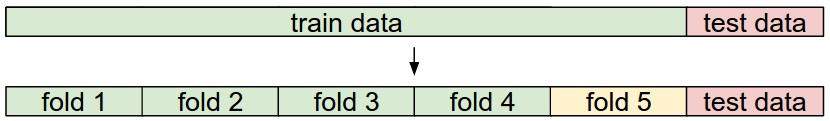
\includegraphics{imgs/crossval.jpeg}
\caption{crossval}
\end{figure}

More detail explanation can be found
\href{http://cs231n.github.io/classification/}{here}.

    \begin{Verbatim}[commandchars=\\\{\}]
{\color{incolor}In [{\color{incolor}17}]:} \PY{k+kn}{import} \PY{n+nn}{copy}
         \PY{n}{num\PYZus{}folds} \PY{o}{=} \PY{l+m+mi}{5}
         \PY{n}{k\PYZus{}choices} \PY{o}{=} \PY{p}{[}\PY{l+m+mi}{1}\PY{p}{,} \PY{l+m+mi}{3}\PY{p}{,} \PY{l+m+mi}{5}\PY{p}{,} \PY{l+m+mi}{8}\PY{p}{,} \PY{l+m+mi}{10}\PY{p}{,} \PY{l+m+mi}{12}\PY{p}{,} \PY{l+m+mi}{15}\PY{p}{,} \PY{l+m+mi}{20}\PY{p}{,} \PY{l+m+mi}{50}\PY{p}{,} \PY{l+m+mi}{100}\PY{p}{]}
         
         \PY{n}{X\PYZus{}train\PYZus{}folds} \PY{o}{=} \PY{p}{[}\PY{p}{]}
         \PY{n}{y\PYZus{}train\PYZus{}folds} \PY{o}{=} \PY{p}{[}\PY{p}{]}
         \PY{c+c1}{\PYZsh{}\PYZsh{}\PYZsh{}\PYZsh{}\PYZsh{}\PYZsh{}\PYZsh{}\PYZsh{}\PYZsh{}\PYZsh{}\PYZsh{}\PYZsh{}\PYZsh{}\PYZsh{}\PYZsh{}\PYZsh{}\PYZsh{}\PYZsh{}\PYZsh{}\PYZsh{}\PYZsh{}\PYZsh{}\PYZsh{}\PYZsh{}\PYZsh{}\PYZsh{}\PYZsh{}\PYZsh{}\PYZsh{}\PYZsh{}\PYZsh{}\PYZsh{}\PYZsh{}\PYZsh{}\PYZsh{}\PYZsh{}\PYZsh{}\PYZsh{}\PYZsh{}\PYZsh{}\PYZsh{}\PYZsh{}\PYZsh{}\PYZsh{}\PYZsh{}\PYZsh{}\PYZsh{}\PYZsh{}\PYZsh{}\PYZsh{}\PYZsh{}\PYZsh{}\PYZsh{}\PYZsh{}\PYZsh{}\PYZsh{}\PYZsh{}\PYZsh{}\PYZsh{}\PYZsh{}\PYZsh{}\PYZsh{}\PYZsh{}\PYZsh{}\PYZsh{}\PYZsh{}\PYZsh{}\PYZsh{}\PYZsh{}\PYZsh{}\PYZsh{}\PYZsh{}\PYZsh{}\PYZsh{}\PYZsh{}\PYZsh{}\PYZsh{}\PYZsh{}\PYZsh{}\PYZsh{}}
         \PY{c+c1}{\PYZsh{} TODO:                                                                        \PYZsh{}}
         \PY{c+c1}{\PYZsh{} Split up the training data into folds. After splitting, X\PYZus{}train\PYZus{}folds and    \PYZsh{}}
         \PY{c+c1}{\PYZsh{} y\PYZus{}train\PYZus{}folds should each be lists of length num\PYZus{}folds, where                \PYZsh{}}
         \PY{c+c1}{\PYZsh{} y\PYZus{}train\PYZus{}folds[i] is the label vector for the points in X\PYZus{}train\PYZus{}folds[i].     \PYZsh{}}
         \PY{c+c1}{\PYZsh{} Hint: Look up the numpy array\PYZus{}split function.                                \PYZsh{}}
         \PY{c+c1}{\PYZsh{}\PYZsh{}\PYZsh{}\PYZsh{}\PYZsh{}\PYZsh{}\PYZsh{}\PYZsh{}\PYZsh{}\PYZsh{}\PYZsh{}\PYZsh{}\PYZsh{}\PYZsh{}\PYZsh{}\PYZsh{}\PYZsh{}\PYZsh{}\PYZsh{}\PYZsh{}\PYZsh{}\PYZsh{}\PYZsh{}\PYZsh{}\PYZsh{}\PYZsh{}\PYZsh{}\PYZsh{}\PYZsh{}\PYZsh{}\PYZsh{}\PYZsh{}\PYZsh{}\PYZsh{}\PYZsh{}\PYZsh{}\PYZsh{}\PYZsh{}\PYZsh{}\PYZsh{}\PYZsh{}\PYZsh{}\PYZsh{}\PYZsh{}\PYZsh{}\PYZsh{}\PYZsh{}\PYZsh{}\PYZsh{}\PYZsh{}\PYZsh{}\PYZsh{}\PYZsh{}\PYZsh{}\PYZsh{}\PYZsh{}\PYZsh{}\PYZsh{}\PYZsh{}\PYZsh{}\PYZsh{}\PYZsh{}\PYZsh{}\PYZsh{}\PYZsh{}\PYZsh{}\PYZsh{}\PYZsh{}\PYZsh{}\PYZsh{}\PYZsh{}\PYZsh{}\PYZsh{}\PYZsh{}\PYZsh{}\PYZsh{}\PYZsh{}\PYZsh{}\PYZsh{}\PYZsh{}}
         \PY{n}{X\PYZus{}train\PYZus{}folds} \PY{o}{=} \PY{n}{np}\PY{o}{.}\PY{n}{array\PYZus{}split}\PY{p}{(}\PY{n}{X\PYZus{}train}\PY{p}{,} \PY{n}{num\PYZus{}folds}\PY{p}{)}
         \PY{n}{y\PYZus{}train\PYZus{}folds} \PY{o}{=} \PY{n}{np}\PY{o}{.}\PY{n}{array\PYZus{}split}\PY{p}{(}\PY{n}{y\PYZus{}train}\PY{p}{,} \PY{n}{num\PYZus{}folds}\PY{p}{)}
         \PY{c+c1}{\PYZsh{}\PYZsh{}\PYZsh{}\PYZsh{}\PYZsh{}\PYZsh{}\PYZsh{}\PYZsh{}\PYZsh{}\PYZsh{}\PYZsh{}\PYZsh{}\PYZsh{}\PYZsh{}\PYZsh{}\PYZsh{}\PYZsh{}\PYZsh{}\PYZsh{}\PYZsh{}\PYZsh{}\PYZsh{}\PYZsh{}\PYZsh{}\PYZsh{}\PYZsh{}\PYZsh{}\PYZsh{}\PYZsh{}\PYZsh{}\PYZsh{}\PYZsh{}\PYZsh{}\PYZsh{}\PYZsh{}\PYZsh{}\PYZsh{}\PYZsh{}\PYZsh{}\PYZsh{}\PYZsh{}\PYZsh{}\PYZsh{}\PYZsh{}\PYZsh{}\PYZsh{}\PYZsh{}\PYZsh{}\PYZsh{}\PYZsh{}\PYZsh{}\PYZsh{}\PYZsh{}\PYZsh{}\PYZsh{}\PYZsh{}\PYZsh{}\PYZsh{}\PYZsh{}\PYZsh{}\PYZsh{}\PYZsh{}\PYZsh{}\PYZsh{}\PYZsh{}\PYZsh{}\PYZsh{}\PYZsh{}\PYZsh{}\PYZsh{}\PYZsh{}\PYZsh{}\PYZsh{}\PYZsh{}\PYZsh{}\PYZsh{}\PYZsh{}\PYZsh{}\PYZsh{}\PYZsh{}}
         \PY{c+c1}{\PYZsh{}                                 END OF YOUR CODE                             \PYZsh{}}
         \PY{c+c1}{\PYZsh{}\PYZsh{}\PYZsh{}\PYZsh{}\PYZsh{}\PYZsh{}\PYZsh{}\PYZsh{}\PYZsh{}\PYZsh{}\PYZsh{}\PYZsh{}\PYZsh{}\PYZsh{}\PYZsh{}\PYZsh{}\PYZsh{}\PYZsh{}\PYZsh{}\PYZsh{}\PYZsh{}\PYZsh{}\PYZsh{}\PYZsh{}\PYZsh{}\PYZsh{}\PYZsh{}\PYZsh{}\PYZsh{}\PYZsh{}\PYZsh{}\PYZsh{}\PYZsh{}\PYZsh{}\PYZsh{}\PYZsh{}\PYZsh{}\PYZsh{}\PYZsh{}\PYZsh{}\PYZsh{}\PYZsh{}\PYZsh{}\PYZsh{}\PYZsh{}\PYZsh{}\PYZsh{}\PYZsh{}\PYZsh{}\PYZsh{}\PYZsh{}\PYZsh{}\PYZsh{}\PYZsh{}\PYZsh{}\PYZsh{}\PYZsh{}\PYZsh{}\PYZsh{}\PYZsh{}\PYZsh{}\PYZsh{}\PYZsh{}\PYZsh{}\PYZsh{}\PYZsh{}\PYZsh{}\PYZsh{}\PYZsh{}\PYZsh{}\PYZsh{}\PYZsh{}\PYZsh{}\PYZsh{}\PYZsh{}\PYZsh{}\PYZsh{}\PYZsh{}\PYZsh{}\PYZsh{}}
         
         \PY{c+c1}{\PYZsh{} A dictionary holding the accuracies for different values of k that we find}
         \PY{c+c1}{\PYZsh{} when running cross\PYZhy{}validation. After running cross\PYZhy{}validation,}
         \PY{c+c1}{\PYZsh{} k\PYZus{}to\PYZus{}accuracies[k] should be a list of length num\PYZus{}folds giving the different}
         \PY{c+c1}{\PYZsh{} accuracy values that we found when using that value of k.}
         \PY{n}{k\PYZus{}to\PYZus{}accuracies} \PY{o}{=} \PY{p}{\PYZob{}}\PY{p}{\PYZcb{}}
         \PY{k}{for} \PY{n}{k\PYZus{}value} \PY{o+ow}{in} \PY{n}{k\PYZus{}choices}\PY{p}{:}
             \PY{n}{k\PYZus{}to\PYZus{}accuracies}\PY{p}{[}\PY{n}{k\PYZus{}value}\PY{p}{]} \PY{o}{=} \PY{p}{[}\PY{p}{]}
             
             \PY{k}{for} \PY{n}{i} \PY{o+ow}{in} \PY{n+nb}{range}\PY{p}{(}\PY{l+m+mi}{5}\PY{p}{)}\PY{p}{:}
                 \PY{n}{Xk\PYZus{}val} \PY{o}{=} \PY{n}{X\PYZus{}train\PYZus{}folds}\PY{p}{[}\PY{n}{i}\PY{p}{]}
                 \PY{n}{yk\PYZus{}val} \PY{o}{=} \PY{n}{y\PYZus{}train\PYZus{}folds}\PY{p}{[}\PY{n}{i}\PY{p}{]}
                 
                 \PY{n}{tempX\PYZus{}train} \PY{o}{=} \PY{n}{copy}\PY{o}{.}\PY{n}{deepcopy}\PY{p}{(}\PY{n}{X\PYZus{}train\PYZus{}folds}\PY{p}{)}
                 \PY{n}{tempy\PYZus{}train} \PY{o}{=} \PY{n}{copy}\PY{o}{.}\PY{n}{deepcopy}\PY{p}{(}\PY{n}{y\PYZus{}train\PYZus{}folds}\PY{p}{)}
                 \PY{k}{del} \PY{n}{tempX\PYZus{}train}\PY{p}{[}\PY{n}{i}\PY{p}{]}
                 \PY{k}{del} \PY{n}{tempy\PYZus{}train}\PY{p}{[}\PY{n}{i}\PY{p}{]}
                 \PY{n}{Xk\PYZus{}train} \PY{o}{=} \PY{n}{np}\PY{o}{.}\PY{n}{concatenate}\PY{p}{(}\PY{n}{tempX\PYZus{}train}\PY{p}{)}
                 \PY{n}{yk\PYZus{}train} \PY{o}{=} \PY{n}{np}\PY{o}{.}\PY{n}{concatenate}\PY{p}{(}\PY{n}{tempy\PYZus{}train}\PY{p}{)}
                 
                 \PY{n}{classifier\PYZus{}k} \PY{o}{=} \PY{n}{KNearestNeighbor}\PY{p}{(}\PY{p}{)}
                 \PY{n}{classifier\PYZus{}k}\PY{o}{.}\PY{n}{train}\PY{p}{(}\PY{n}{Xk\PYZus{}train}\PY{p}{,} \PY{n}{yk\PYZus{}train}\PY{p}{)}
                 
                 \PY{n}{dists} \PY{o}{=} \PY{n}{classifier\PYZus{}k}\PY{o}{.}\PY{n}{compute\PYZus{}distances\PYZus{}no\PYZus{}loops}\PY{p}{(}\PY{n}{Xk\PYZus{}val}\PY{p}{)}
                 \PY{n}{y\PYZus{}test\PYZus{}pred} \PY{o}{=} \PY{n}{classifier\PYZus{}k}\PY{o}{.}\PY{n}{predict\PYZus{}labels}\PY{p}{(}\PY{n}{dists}\PY{p}{,} \PY{n}{k}\PY{o}{=}\PY{n}{k\PYZus{}value}\PY{p}{)}
                 \PY{n}{num\PYZus{}correct} \PY{o}{=} \PY{n}{np}\PY{o}{.}\PY{n}{sum}\PY{p}{(}\PY{n}{y\PYZus{}test\PYZus{}pred} \PY{o}{==} \PY{n}{yk\PYZus{}val}\PY{p}{)}
                 \PY{n}{accuracy} \PY{o}{=} \PY{n+nb}{float}\PY{p}{(}\PY{n}{num\PYZus{}correct}\PY{p}{)} \PY{o}{/} \PY{n+nb}{len}\PY{p}{(}\PY{n}{Xk\PYZus{}val}\PY{p}{)}
                 \PY{n}{k\PYZus{}to\PYZus{}accuracies}\PY{p}{[}\PY{n}{k\PYZus{}value}\PY{p}{]}\PY{o}{.}\PY{n}{append}\PY{p}{(}\PY{n}{accuracy}\PY{p}{)}
         
         \PY{c+c1}{\PYZsh{}\PYZsh{}\PYZsh{}\PYZsh{}\PYZsh{}\PYZsh{}\PYZsh{}\PYZsh{}\PYZsh{}\PYZsh{}\PYZsh{}\PYZsh{}\PYZsh{}\PYZsh{}\PYZsh{}\PYZsh{}\PYZsh{}\PYZsh{}\PYZsh{}\PYZsh{}\PYZsh{}\PYZsh{}\PYZsh{}\PYZsh{}\PYZsh{}\PYZsh{}\PYZsh{}\PYZsh{}\PYZsh{}\PYZsh{}\PYZsh{}\PYZsh{}\PYZsh{}\PYZsh{}\PYZsh{}\PYZsh{}\PYZsh{}\PYZsh{}\PYZsh{}\PYZsh{}\PYZsh{}\PYZsh{}\PYZsh{}\PYZsh{}\PYZsh{}\PYZsh{}\PYZsh{}\PYZsh{}\PYZsh{}\PYZsh{}\PYZsh{}\PYZsh{}\PYZsh{}\PYZsh{}\PYZsh{}\PYZsh{}\PYZsh{}\PYZsh{}\PYZsh{}\PYZsh{}\PYZsh{}\PYZsh{}\PYZsh{}\PYZsh{}\PYZsh{}\PYZsh{}\PYZsh{}\PYZsh{}\PYZsh{}\PYZsh{}\PYZsh{}\PYZsh{}\PYZsh{}\PYZsh{}\PYZsh{}\PYZsh{}\PYZsh{}\PYZsh{}\PYZsh{}\PYZsh{}}
         \PY{c+c1}{\PYZsh{} TODO:                                                                        \PYZsh{}}
         \PY{c+c1}{\PYZsh{} Perform k\PYZhy{}fold cross validation to find the best value of k. For each        \PYZsh{}}
         \PY{c+c1}{\PYZsh{} possible value of k, run the k\PYZhy{}nearest\PYZhy{}neighbor algorithm num\PYZus{}folds times,   \PYZsh{}}
         \PY{c+c1}{\PYZsh{} where in each case you use all but one of the folds as training data and the \PYZsh{}}
         \PY{c+c1}{\PYZsh{} last fold as a validation set. Store the accuracies for all fold and all     \PYZsh{}}
         \PY{c+c1}{\PYZsh{} values of k in the k\PYZus{}to\PYZus{}accuracies dictionary.                               \PYZsh{}}
         \PY{c+c1}{\PYZsh{}\PYZsh{}\PYZsh{}\PYZsh{}\PYZsh{}\PYZsh{}\PYZsh{}\PYZsh{}\PYZsh{}\PYZsh{}\PYZsh{}\PYZsh{}\PYZsh{}\PYZsh{}\PYZsh{}\PYZsh{}\PYZsh{}\PYZsh{}\PYZsh{}\PYZsh{}\PYZsh{}\PYZsh{}\PYZsh{}\PYZsh{}\PYZsh{}\PYZsh{}\PYZsh{}\PYZsh{}\PYZsh{}\PYZsh{}\PYZsh{}\PYZsh{}\PYZsh{}\PYZsh{}\PYZsh{}\PYZsh{}\PYZsh{}\PYZsh{}\PYZsh{}\PYZsh{}\PYZsh{}\PYZsh{}\PYZsh{}\PYZsh{}\PYZsh{}\PYZsh{}\PYZsh{}\PYZsh{}\PYZsh{}\PYZsh{}\PYZsh{}\PYZsh{}\PYZsh{}\PYZsh{}\PYZsh{}\PYZsh{}\PYZsh{}\PYZsh{}\PYZsh{}\PYZsh{}\PYZsh{}\PYZsh{}\PYZsh{}\PYZsh{}\PYZsh{}\PYZsh{}\PYZsh{}\PYZsh{}\PYZsh{}\PYZsh{}\PYZsh{}\PYZsh{}\PYZsh{}\PYZsh{}\PYZsh{}\PYZsh{}\PYZsh{}\PYZsh{}\PYZsh{}\PYZsh{}}
         
         \PY{c+c1}{\PYZsh{}\PYZsh{}\PYZsh{}\PYZsh{}\PYZsh{}\PYZsh{}\PYZsh{}\PYZsh{}\PYZsh{}\PYZsh{}\PYZsh{}\PYZsh{}\PYZsh{}\PYZsh{}\PYZsh{}\PYZsh{}\PYZsh{}\PYZsh{}\PYZsh{}\PYZsh{}\PYZsh{}\PYZsh{}\PYZsh{}\PYZsh{}\PYZsh{}\PYZsh{}\PYZsh{}\PYZsh{}\PYZsh{}\PYZsh{}\PYZsh{}\PYZsh{}\PYZsh{}\PYZsh{}\PYZsh{}\PYZsh{}\PYZsh{}\PYZsh{}\PYZsh{}\PYZsh{}\PYZsh{}\PYZsh{}\PYZsh{}\PYZsh{}\PYZsh{}\PYZsh{}\PYZsh{}\PYZsh{}\PYZsh{}\PYZsh{}\PYZsh{}\PYZsh{}\PYZsh{}\PYZsh{}\PYZsh{}\PYZsh{}\PYZsh{}\PYZsh{}\PYZsh{}\PYZsh{}\PYZsh{}\PYZsh{}\PYZsh{}\PYZsh{}\PYZsh{}\PYZsh{}\PYZsh{}\PYZsh{}\PYZsh{}\PYZsh{}\PYZsh{}\PYZsh{}\PYZsh{}\PYZsh{}\PYZsh{}\PYZsh{}\PYZsh{}\PYZsh{}\PYZsh{}\PYZsh{}}
         \PY{c+c1}{\PYZsh{}                                 END OF YOUR CODE                             \PYZsh{}}
         \PY{c+c1}{\PYZsh{}\PYZsh{}\PYZsh{}\PYZsh{}\PYZsh{}\PYZsh{}\PYZsh{}\PYZsh{}\PYZsh{}\PYZsh{}\PYZsh{}\PYZsh{}\PYZsh{}\PYZsh{}\PYZsh{}\PYZsh{}\PYZsh{}\PYZsh{}\PYZsh{}\PYZsh{}\PYZsh{}\PYZsh{}\PYZsh{}\PYZsh{}\PYZsh{}\PYZsh{}\PYZsh{}\PYZsh{}\PYZsh{}\PYZsh{}\PYZsh{}\PYZsh{}\PYZsh{}\PYZsh{}\PYZsh{}\PYZsh{}\PYZsh{}\PYZsh{}\PYZsh{}\PYZsh{}\PYZsh{}\PYZsh{}\PYZsh{}\PYZsh{}\PYZsh{}\PYZsh{}\PYZsh{}\PYZsh{}\PYZsh{}\PYZsh{}\PYZsh{}\PYZsh{}\PYZsh{}\PYZsh{}\PYZsh{}\PYZsh{}\PYZsh{}\PYZsh{}\PYZsh{}\PYZsh{}\PYZsh{}\PYZsh{}\PYZsh{}\PYZsh{}\PYZsh{}\PYZsh{}\PYZsh{}\PYZsh{}\PYZsh{}\PYZsh{}\PYZsh{}\PYZsh{}\PYZsh{}\PYZsh{}\PYZsh{}\PYZsh{}\PYZsh{}\PYZsh{}\PYZsh{}\PYZsh{}}
         
         \PY{c+c1}{\PYZsh{} Print out the computed accuracies}
         \PY{k}{for} \PY{n}{k} \PY{o+ow}{in} \PY{n+nb}{sorted}\PY{p}{(}\PY{n}{k\PYZus{}to\PYZus{}accuracies}\PY{p}{)}\PY{p}{:}
             \PY{k}{for} \PY{n}{accuracy} \PY{o+ow}{in} \PY{n}{k\PYZus{}to\PYZus{}accuracies}\PY{p}{[}\PY{n}{k}\PY{p}{]}\PY{p}{:}
                 \PY{n+nb}{print} \PY{p}{(}\PY{l+s+s1}{\PYZsq{}}\PY{l+s+s1}{k = }\PY{l+s+si}{\PYZpc{}d}\PY{l+s+s1}{, accuracy = }\PY{l+s+si}{\PYZpc{}f}\PY{l+s+s1}{\PYZsq{}} \PY{o}{\PYZpc{}} \PY{p}{(}\PY{n}{k}\PY{p}{,} \PY{n}{accuracy}\PY{p}{)}\PY{p}{)}
\end{Verbatim}


    \begin{Verbatim}[commandchars=\\\{\}]
k = 1, accuracy = 0.263000
k = 1, accuracy = 0.257000
k = 1, accuracy = 0.264000
k = 1, accuracy = 0.278000
k = 1, accuracy = 0.266000
k = 3, accuracy = 0.241000
k = 3, accuracy = 0.249000
k = 3, accuracy = 0.243000
k = 3, accuracy = 0.273000
k = 3, accuracy = 0.264000
k = 5, accuracy = 0.256000
k = 5, accuracy = 0.271000
k = 5, accuracy = 0.280000
k = 5, accuracy = 0.289000
k = 5, accuracy = 0.278000
k = 8, accuracy = 0.263000
k = 8, accuracy = 0.287000
k = 8, accuracy = 0.276000
k = 8, accuracy = 0.288000
k = 8, accuracy = 0.270000
k = 10, accuracy = 0.266000
k = 10, accuracy = 0.296000
k = 10, accuracy = 0.279000
k = 10, accuracy = 0.283000
k = 10, accuracy = 0.283000
k = 12, accuracy = 0.261000
k = 12, accuracy = 0.294000
k = 12, accuracy = 0.280000
k = 12, accuracy = 0.283000
k = 12, accuracy = 0.280000
k = 15, accuracy = 0.253000
k = 15, accuracy = 0.290000
k = 15, accuracy = 0.279000
k = 15, accuracy = 0.280000
k = 15, accuracy = 0.275000
k = 20, accuracy = 0.270000
k = 20, accuracy = 0.279000
k = 20, accuracy = 0.279000
k = 20, accuracy = 0.280000
k = 20, accuracy = 0.284000
k = 50, accuracy = 0.271000
k = 50, accuracy = 0.288000
k = 50, accuracy = 0.278000
k = 50, accuracy = 0.269000
k = 50, accuracy = 0.266000
k = 100, accuracy = 0.256000
k = 100, accuracy = 0.270000
k = 100, accuracy = 0.263000
k = 100, accuracy = 0.256000
k = 100, accuracy = 0.263000

    \end{Verbatim}

    \begin{Verbatim}[commandchars=\\\{\}]
{\color{incolor}In [{\color{incolor}18}]:} \PY{c+c1}{\PYZsh{} plot the raw observations}
         \PY{k}{for} \PY{n}{k} \PY{o+ow}{in} \PY{n}{k\PYZus{}choices}\PY{p}{:}
             \PY{n}{accuracies} \PY{o}{=} \PY{n}{k\PYZus{}to\PYZus{}accuracies}\PY{p}{[}\PY{n}{k}\PY{p}{]}
             \PY{n}{plt}\PY{o}{.}\PY{n}{scatter}\PY{p}{(}\PY{p}{[}\PY{n}{k}\PY{p}{]} \PY{o}{*} \PY{n+nb}{len}\PY{p}{(}\PY{n}{accuracies}\PY{p}{)}\PY{p}{,} \PY{n}{accuracies}\PY{p}{)}
         
         \PY{c+c1}{\PYZsh{} plot the trend line with error bars that correspond to standard deviation}
         \PY{n}{accuracies\PYZus{}mean} \PY{o}{=} \PY{n}{np}\PY{o}{.}\PY{n}{array}\PY{p}{(}\PY{p}{[}\PY{n}{np}\PY{o}{.}\PY{n}{mean}\PY{p}{(}\PY{n}{v}\PY{p}{)} \PY{k}{for} \PY{n}{k}\PY{p}{,}\PY{n}{v} \PY{o+ow}{in} \PY{n+nb}{sorted}\PY{p}{(}\PY{n}{k\PYZus{}to\PYZus{}accuracies}\PY{o}{.}\PY{n}{items}\PY{p}{(}\PY{p}{)}\PY{p}{)}\PY{p}{]}\PY{p}{)}
         \PY{n}{accuracies\PYZus{}std} \PY{o}{=} \PY{n}{np}\PY{o}{.}\PY{n}{array}\PY{p}{(}\PY{p}{[}\PY{n}{np}\PY{o}{.}\PY{n}{std}\PY{p}{(}\PY{n}{v}\PY{p}{)} \PY{k}{for} \PY{n}{k}\PY{p}{,}\PY{n}{v} \PY{o+ow}{in} \PY{n+nb}{sorted}\PY{p}{(}\PY{n}{k\PYZus{}to\PYZus{}accuracies}\PY{o}{.}\PY{n}{items}\PY{p}{(}\PY{p}{)}\PY{p}{)}\PY{p}{]}\PY{p}{)}
         \PY{n}{plt}\PY{o}{.}\PY{n}{errorbar}\PY{p}{(}\PY{n}{k\PYZus{}choices}\PY{p}{,} \PY{n}{accuracies\PYZus{}mean}\PY{p}{,} \PY{n}{yerr}\PY{o}{=}\PY{n}{accuracies\PYZus{}std}\PY{p}{)}
         \PY{n}{plt}\PY{o}{.}\PY{n}{title}\PY{p}{(}\PY{l+s+s1}{\PYZsq{}}\PY{l+s+s1}{Cross\PYZhy{}validation on k}\PY{l+s+s1}{\PYZsq{}}\PY{p}{)}
         \PY{n}{plt}\PY{o}{.}\PY{n}{xlabel}\PY{p}{(}\PY{l+s+s1}{\PYZsq{}}\PY{l+s+s1}{k}\PY{l+s+s1}{\PYZsq{}}\PY{p}{)}
         \PY{n}{plt}\PY{o}{.}\PY{n}{ylabel}\PY{p}{(}\PY{l+s+s1}{\PYZsq{}}\PY{l+s+s1}{Cross\PYZhy{}validation accuracy}\PY{l+s+s1}{\PYZsq{}}\PY{p}{)}
         \PY{n}{plt}\PY{o}{.}\PY{n}{show}\PY{p}{(}\PY{p}{)}
\end{Verbatim}


    \begin{center}
    \adjustimage{max size={0.9\linewidth}{0.9\paperheight}}{output_25_0.png}
    \end{center}
    { \hspace*{\fill} \\}
    
    \begin{Verbatim}[commandchars=\\\{\}]
{\color{incolor}In [{\color{incolor}19}]:} \PY{c+c1}{\PYZsh{} Based on the cross\PYZhy{}validation results above, choose the best value for k,   }
         \PY{c+c1}{\PYZsh{} retrain the classifier using all the training data, and test it on the test}
         \PY{c+c1}{\PYZsh{} data. You should be able to get above 10\PYZpc{} accuracy on the test data.}
         \PY{n}{best\PYZus{}k} \PY{o}{=} \PY{l+m+mi}{10}
         
         \PY{n}{classifier} \PY{o}{=} \PY{n}{KNearestNeighbor}\PY{p}{(}\PY{p}{)}
         \PY{n}{classifier}\PY{o}{.}\PY{n}{train}\PY{p}{(}\PY{n}{X\PYZus{}train}\PY{p}{,} \PY{n}{y\PYZus{}train}\PY{p}{)}
         \PY{n}{y\PYZus{}test\PYZus{}pred} \PY{o}{=} \PY{n}{classifier}\PY{o}{.}\PY{n}{predict}\PY{p}{(}\PY{n}{X\PYZus{}test}\PY{p}{,} \PY{n}{k}\PY{o}{=}\PY{n}{best\PYZus{}k}\PY{p}{,} \PY{n}{num\PYZus{}loops} \PY{o}{=} \PY{l+m+mi}{0}\PY{p}{)}
         
         \PY{c+c1}{\PYZsh{} Compute and display the accuracy}
         \PY{n}{num\PYZus{}correct} \PY{o}{=} \PY{n}{np}\PY{o}{.}\PY{n}{sum}\PY{p}{(}\PY{n}{y\PYZus{}test\PYZus{}pred} \PY{o}{==} \PY{n}{y\PYZus{}test}\PY{p}{)}
         \PY{n}{accuracy} \PY{o}{=} \PY{n+nb}{float}\PY{p}{(}\PY{n}{num\PYZus{}correct}\PY{p}{)} \PY{o}{/} \PY{n}{num\PYZus{}test}
         \PY{n+nb}{print} \PY{p}{(}\PY{l+s+s1}{\PYZsq{}}\PY{l+s+s1}{Got }\PY{l+s+si}{\PYZpc{}d}\PY{l+s+s1}{ / }\PY{l+s+si}{\PYZpc{}d}\PY{l+s+s1}{ correct =\PYZgt{} accuracy: }\PY{l+s+si}{\PYZpc{}f}\PY{l+s+s1}{\PYZsq{}} \PY{o}{\PYZpc{}} \PY{p}{(}\PY{n}{num\PYZus{}correct}\PY{p}{,} \PY{n}{num\PYZus{}test}\PY{p}{,} \PY{n}{accuracy}\PY{p}{)}\PY{p}{)}
\end{Verbatim}


    \begin{Verbatim}[commandchars=\\\{\}]
Got 141 / 500 correct => accuracy: 0.282000

    \end{Verbatim}


    % Add a bibliography block to the postdoc
    
    
    
    \end{document}
